\section{Snímanie}
\label{sec:Practice-Capturing}

Aplikácia generuje HDR obsah kombinovaním LDR fotografií s rôznou hodnotou času expozície.
Snímanie fotografií je implementované nad aplikačým rozhraním
Camera2\footnote{\url{https://developer.android.com/reference/android/hardware/camera2/package-summary.html}}
operačného systému Android. Aplikácii, pracujúcej s týmto rozhraním, musí byť užívateľom udelené povolenie 
\texttt{android.permission.CAMERA}.

Po inicializovaní obrazovky (obr. \ref{fig:sketch_capture}) sa vytvorí inštancia \texttt{CameraManager}, ktorá poskytuje
detekciu, charakterizáciu a pripojenie k dostupným \texttt{CameraDevices} \cite{Android}.
Každá z~\texttt{CameraDevices} obsahuje súbor vlastností a nastavení snímača, ku ktorým pristupujeme pomocou
objektu \texttt{CameraCharacteristics}.

Následne je vytvorená \texttt{CameraCaptureSession}, ktorej zvolíme výstupnú oblasť \texttt{Surface}. 
Pre zobrazovanie scény v reálnom čase zobrazujeme na výstup stream záberov scény, ktorý dosiahneme nastavením
opakovaného požiadavku o snímanie. \texttt{CaptureRequest} (požiadavok o~snímanie) vytvárame nastavovaním parametrov
objektu \texttt{CaptureRequest.Builder}. Pri zobrazovaní náhľadu užívateľovi využijeme automatické nastavenia
parametrov snímania (\texttt{CONTROL\_MODE\_AUTO}). Do vytvoreného požiadavku o stream záberov scény vložíme callback
\texttt{CaptureCallback}, ktorého metóda \texttt{onCaptureCompleted} vracia objekt typu \texttt{TotalCaptureResult}.
Tento objekt obsahuje hodnoty konfigurácie snímača zariadenia, po~vytvorení posledného snímku. Z tejto
konfigurácie následne získavame hodnoty času expozície, ISO, clony a korekcie farieb, ktoré sú automaticky zvolené
snímačom. Hodnoty ukladáme do premenných, ktoré neskôr použijeme pri manuálnych nastaveniach snímania. Keďže táto
operácia nie je časovo ani priestorovo náročná a nenarúša plynulé zobrazenie streamu scény a taktiež hodnoty
senzora sa menia vplyvom scény, sú tieto hodnoty nastavované v každom \texttt{CaptureCallback}u po uskutočnení
požiadavku o snímanie.

Ak užívateľ stlačí tlačidlo pre snímanie scény, je zastavené opakovanie požiadavku zobrazovania streamu.
V tomto okamihu je potrebné vytvoriť sériu záberov scény, s manuálne nastavenými hodnotami parametrov.
Dosiahneme to definovaním zoznamu požiadavkov o~snímanie, ktoré budú mať špecifikované hodnoty parametrov.
Pre nastavovanie vlastných parametrov, musí byť aktivovaný manuálny mód a to vypnutím \texttt{CONTROL\_MODE}.
Hodnoty parametrov ako citlivosť snímača (ISO) a clona sú nájdené ako najvhodnejšia kombinácia 
pre najlepší výsledok. Najdôležitejším parametrom je však dĺžka času expozície v nanosekundách,
počas ktorého je snímač vystavený svetlu z prostredia scény.
Zoznam požiadavkov o vytvorenie snímok s manuálnymi parametrami je poslaný do metódy \texttt{captureBurst()}.
Zachytený snímok sa v callbacku \texttt{OnImageAvailableListener} spracuje a vloží do zoznamu k ostatným záberom 
danej scény.

\subsection{Nastavenie času expozície}
\label{sec:Practice-ExpoSelector}

Ako už bolo spomínané, vybrané \texttt{CameraDevice} nám poskytuje vlastnosti snímača, popísané 
v \texttt{CameraCharacteristics} \cite{Android}. Odtiaľ získame aj rozsah povoleného expozičného času snímača 
\texttt{SENSOR\_INFO\_EXPOSURE\_TIME\_RANGE}. Tento rozsah využijeme pri výpočte expozičných časov,
ktoré budú využité pri snímaní. V mnohých zdrojoch sa uvádzajú odporúčané časy expozície vyjadrené ako
hodnoty geometrického radu - každý čas expozície je konštantným násobkom predchadzajúceho času.

Trieda \texttt{Exposures} pomocou postupne získaných informácií o rozsahu povoleného expozičného času snímača
a automaticky zvolenej hodnoty času expozície v aktuálnej scéne vytvára zoznam vybraných expozičných časov pre manuálne
nastavenia. Pri inicializovaní snímača zariadenia a získania rozsahu expozičných časov sú do zoznamu \texttt{range}
postupne vkladané hodnoty času expozície v tvare $2^{n}$ nanosekúnd. V okamihu, keď nastane stav manuálneho snímania scény,
vytvorí sa zoznam vybraných expozičných časov, ktorých strednou hodnotou je hodnota automatickej expozície (obr. \ref{fig:expoSelector0}).
Povolený rozsah expozičného času však nemusí umožňovať, aby prostrednou hodnotou bola práve táto hodnota (obr. \ref{fig:expoSelector1}). 
Pre~riešenie týchto problémov bol vytvorený krátky algoritmus popísaný v pseudokóde \ref{algo_expositions}.

Algoritmus vytvára zoznam hodnôt geometrického radu v tvare $2^{n}$ $ns$ v povolenom rozsahu.
V tomto zozname sa zvolí hodnota najbližia hodnote automatickej expozície ako prostredná hodnota
a vo zvolenom kroku sa striedavo hľadajú hodnoty nižšie od strednej hodnoty a hodnoty vyššie.
Algoritmus končí, ak konečný zoznam obsahuje zvolený počet expozičných časov, alebo ak nie je
možné nájsť ďalšiu hodnotu.

\begin{figure}[h!]
    \centering
    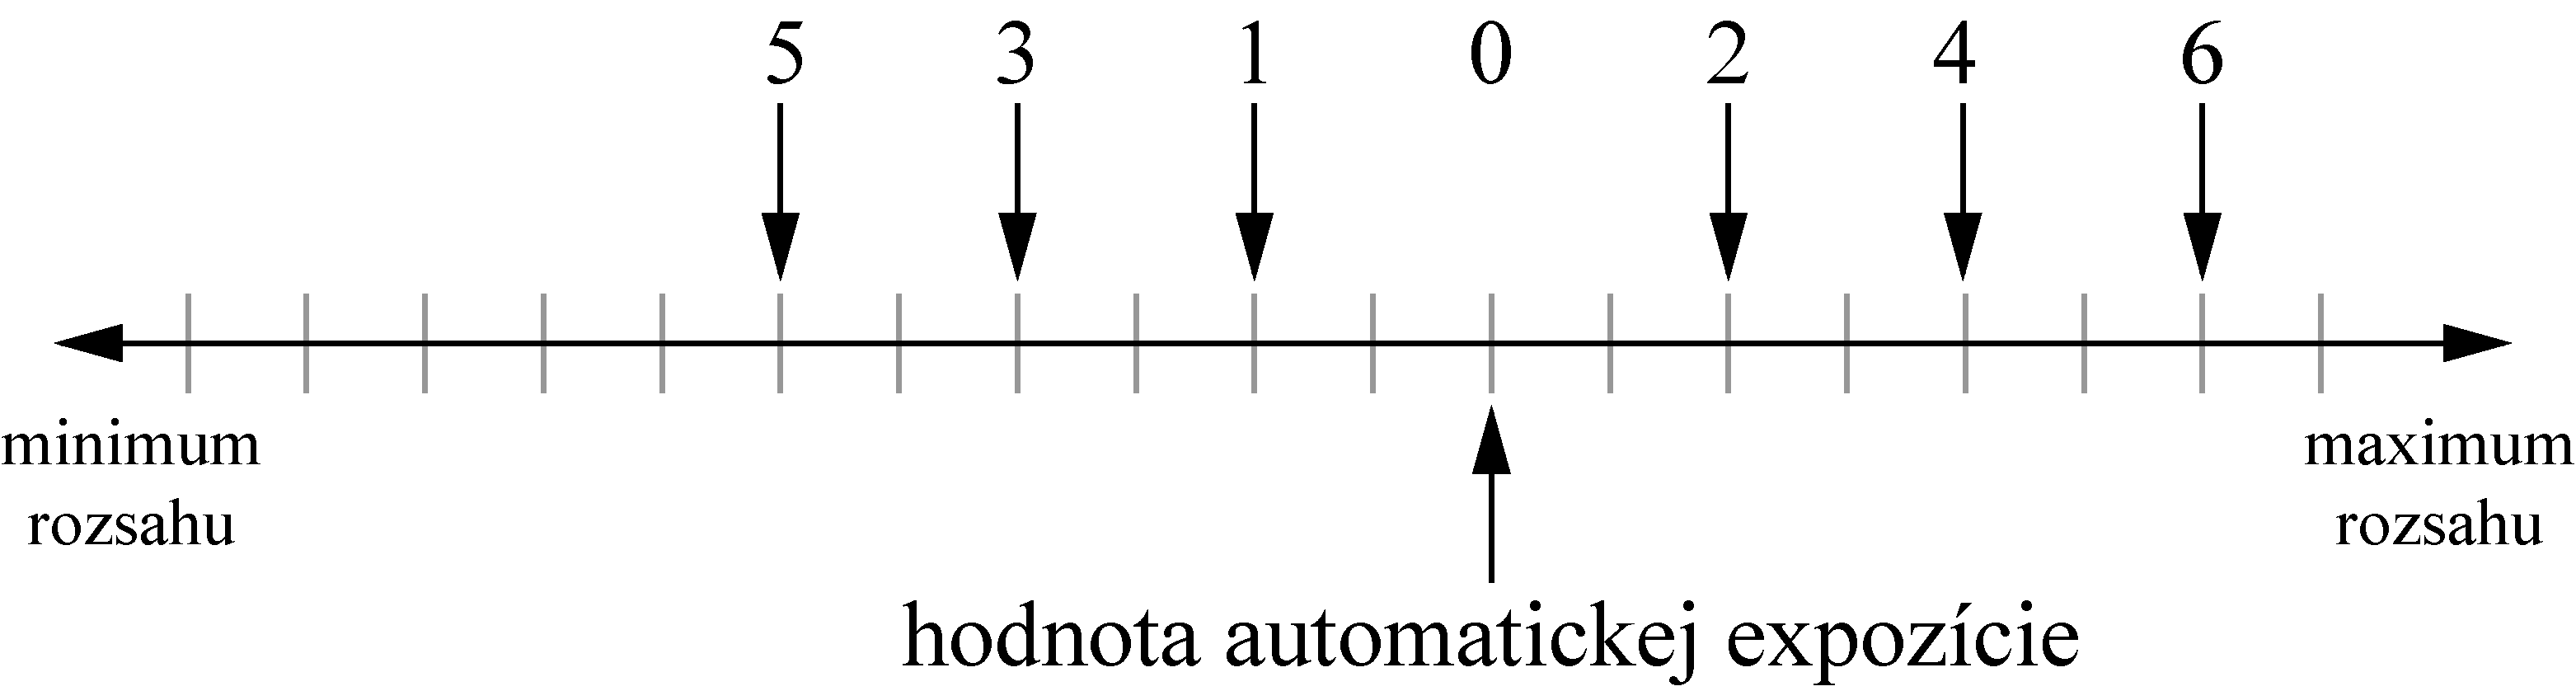
\includegraphics[width=0.7\textwidth]{figures/capturing/expoSelector0}
    \caption{Vyhľadávanie vhodných hodnôt časov expozície s krokom 2 (čísla zobrazujú poradie nájdených hodnôt)}
    \label{fig:expoSelector0}
\end{figure}

\begin{figure}[h!]
    \centering
    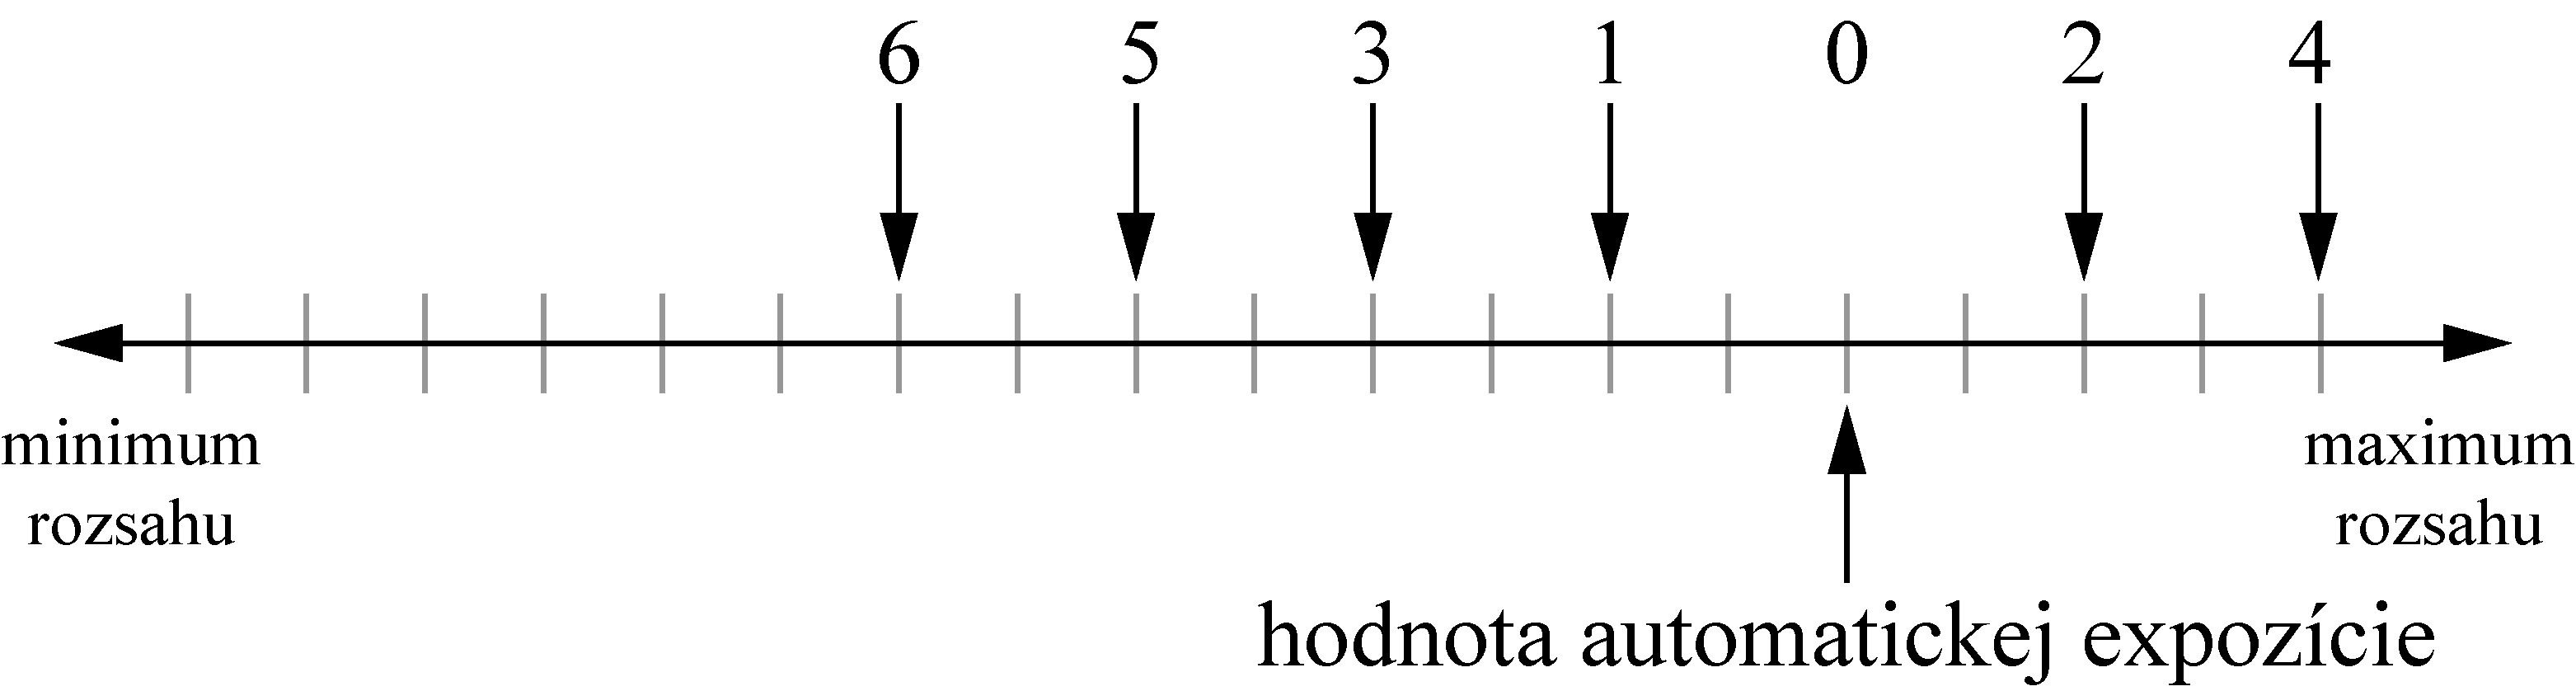
\includegraphics[width=0.7\textwidth]{figures/capturing/expoSelector1}
    \caption{Riešenie problému pri vysokej hodnote automatickej expozície}
    \label{fig:expoSelector1}
\end{figure}

\begin{algorithm}[]
    \SetAlgoLined
    \DontPrintSemicolon
    \caption{Výber expozičných časov}
    \label{algo_expositions}

    vstupy algoritmu:\;
    \texttt{  maxExpo} - maximálny počet expozícii\;
    \texttt{  krok} - krok pri výbere medzi expozičnými časmi v zozname \texttt{range}\;
    \texttt{  stredExpo} - hodnota automatickej expozície (najbližšia hodnota v tvare $2^{n}$)\;
    \;
    inicializácia premenných:\;
    \texttt{  stredIdx} = index hodnoty \texttt{stredExpo} v zozname \texttt{range}\;
    \texttt{  mensiIdx} = \texttt{stredIdx - krok}\;
    \texttt{  vacsiIdx} = \texttt{stredIdx + krok}\;
    \texttt{  pocet} - počet hodnôt v zozname \texttt{exposures}\;
    \texttt{  vacsiaHodnota} - booleanovská hodnota značiaca, či sa bude vyhľadávať menšia,
    alebo väčšia hodnota času expozície\;
    \texttt{  najdene} - booleanovská hodnota značiaca či sa v predchadzajúcom cykle našla vhodná hodnota\;
    \;
    vlož \texttt{stredExpo} do zoznamu \texttt{expozicie};\;
    \;
    \While{pocet < maxExpo}{
        \eIf{vacsiaHodnota}{
            \eIf{vacsiIdx <= najväčší index zoznamu range}{
                vlož hodnotu na indexe \texttt{vacsiIdx} zo zoznamu \texttt{range} do zoznamu \texttt{expozicie};\;
                \texttt{najdene} nastav na true;\;
                \texttt{vacsiIdx} inkrementuj o \texttt{krok};\;
                inkrementuj \texttt{pocet};\;
            }{
                ak sa v predchádzajúcom cykle nenašla vhodná hodnota - ukonči algoritmus;\;
                \texttt{najdene} nastav na false;\;
            }
            \texttt{vacsiaHodnota} nastav na false;\;
        }{
            \eIf{mensiIdx >= 0}{
                vlož hodnotu na indexe \texttt{mensiIdx} zo zoznamu \texttt{range} do zoznamu \texttt{expozicie};\;
                \texttt{najdene} nastav na true;\;
                \texttt{vacsiIdx} dekrementuj o \texttt{krok};\;
                inkrementuj \texttt{pocet};\;
            }{
                ak sa v predchádzajúcom cykle nenašla vhodná hodnota - ukonči algoritmus;\;
                \texttt{najdene} nastav na false;\;
            }
            \texttt{vacsiaHodnota} nastav na true;\;
        }
    }
\end{algorithm}

\subsection{Zarovnanie}
\label{sec:Practice-Alignment}

Jedným z predpokladov vytvárania HDR obsahu je statickosť zariadenia medzi fotografovaním jednotlivých expozícií.
Profesionálny fotograf si za normálnych okolností pri vytváraní HDR fotografie nasadí fotoaparát na statív.
Fotografovia používajú taktiež funkciu zvanú predsklopenie zrkadla (MLU\footnote{Mirror lock-up}) pre zníženie 
ďalších vibrácií. Problémy so zarovnaním sú oveľa horšie, ak sú zábery fotografované fotoaparátom vo voľnej ruke, 
alebo ako v našom prípade - fotografovaním pomocou smartfónu či tabletu.

Nezarovnanie snímok použitých pri vytváraní HDR obrazu môže mať za následok vážne artefakty. Na obrázku
\ref{fig:unaligned} môžeme vidieť artefakty nazývané ghosting (duchovia), ktoré majú vplyv na výsledný
obrázok. Ghosting nastáva aj v prípade, že sa na statickej scéne nachádza objekt, ktorý je voči scéne v pohybe.

\begin{figure}[h!]
    \centering
    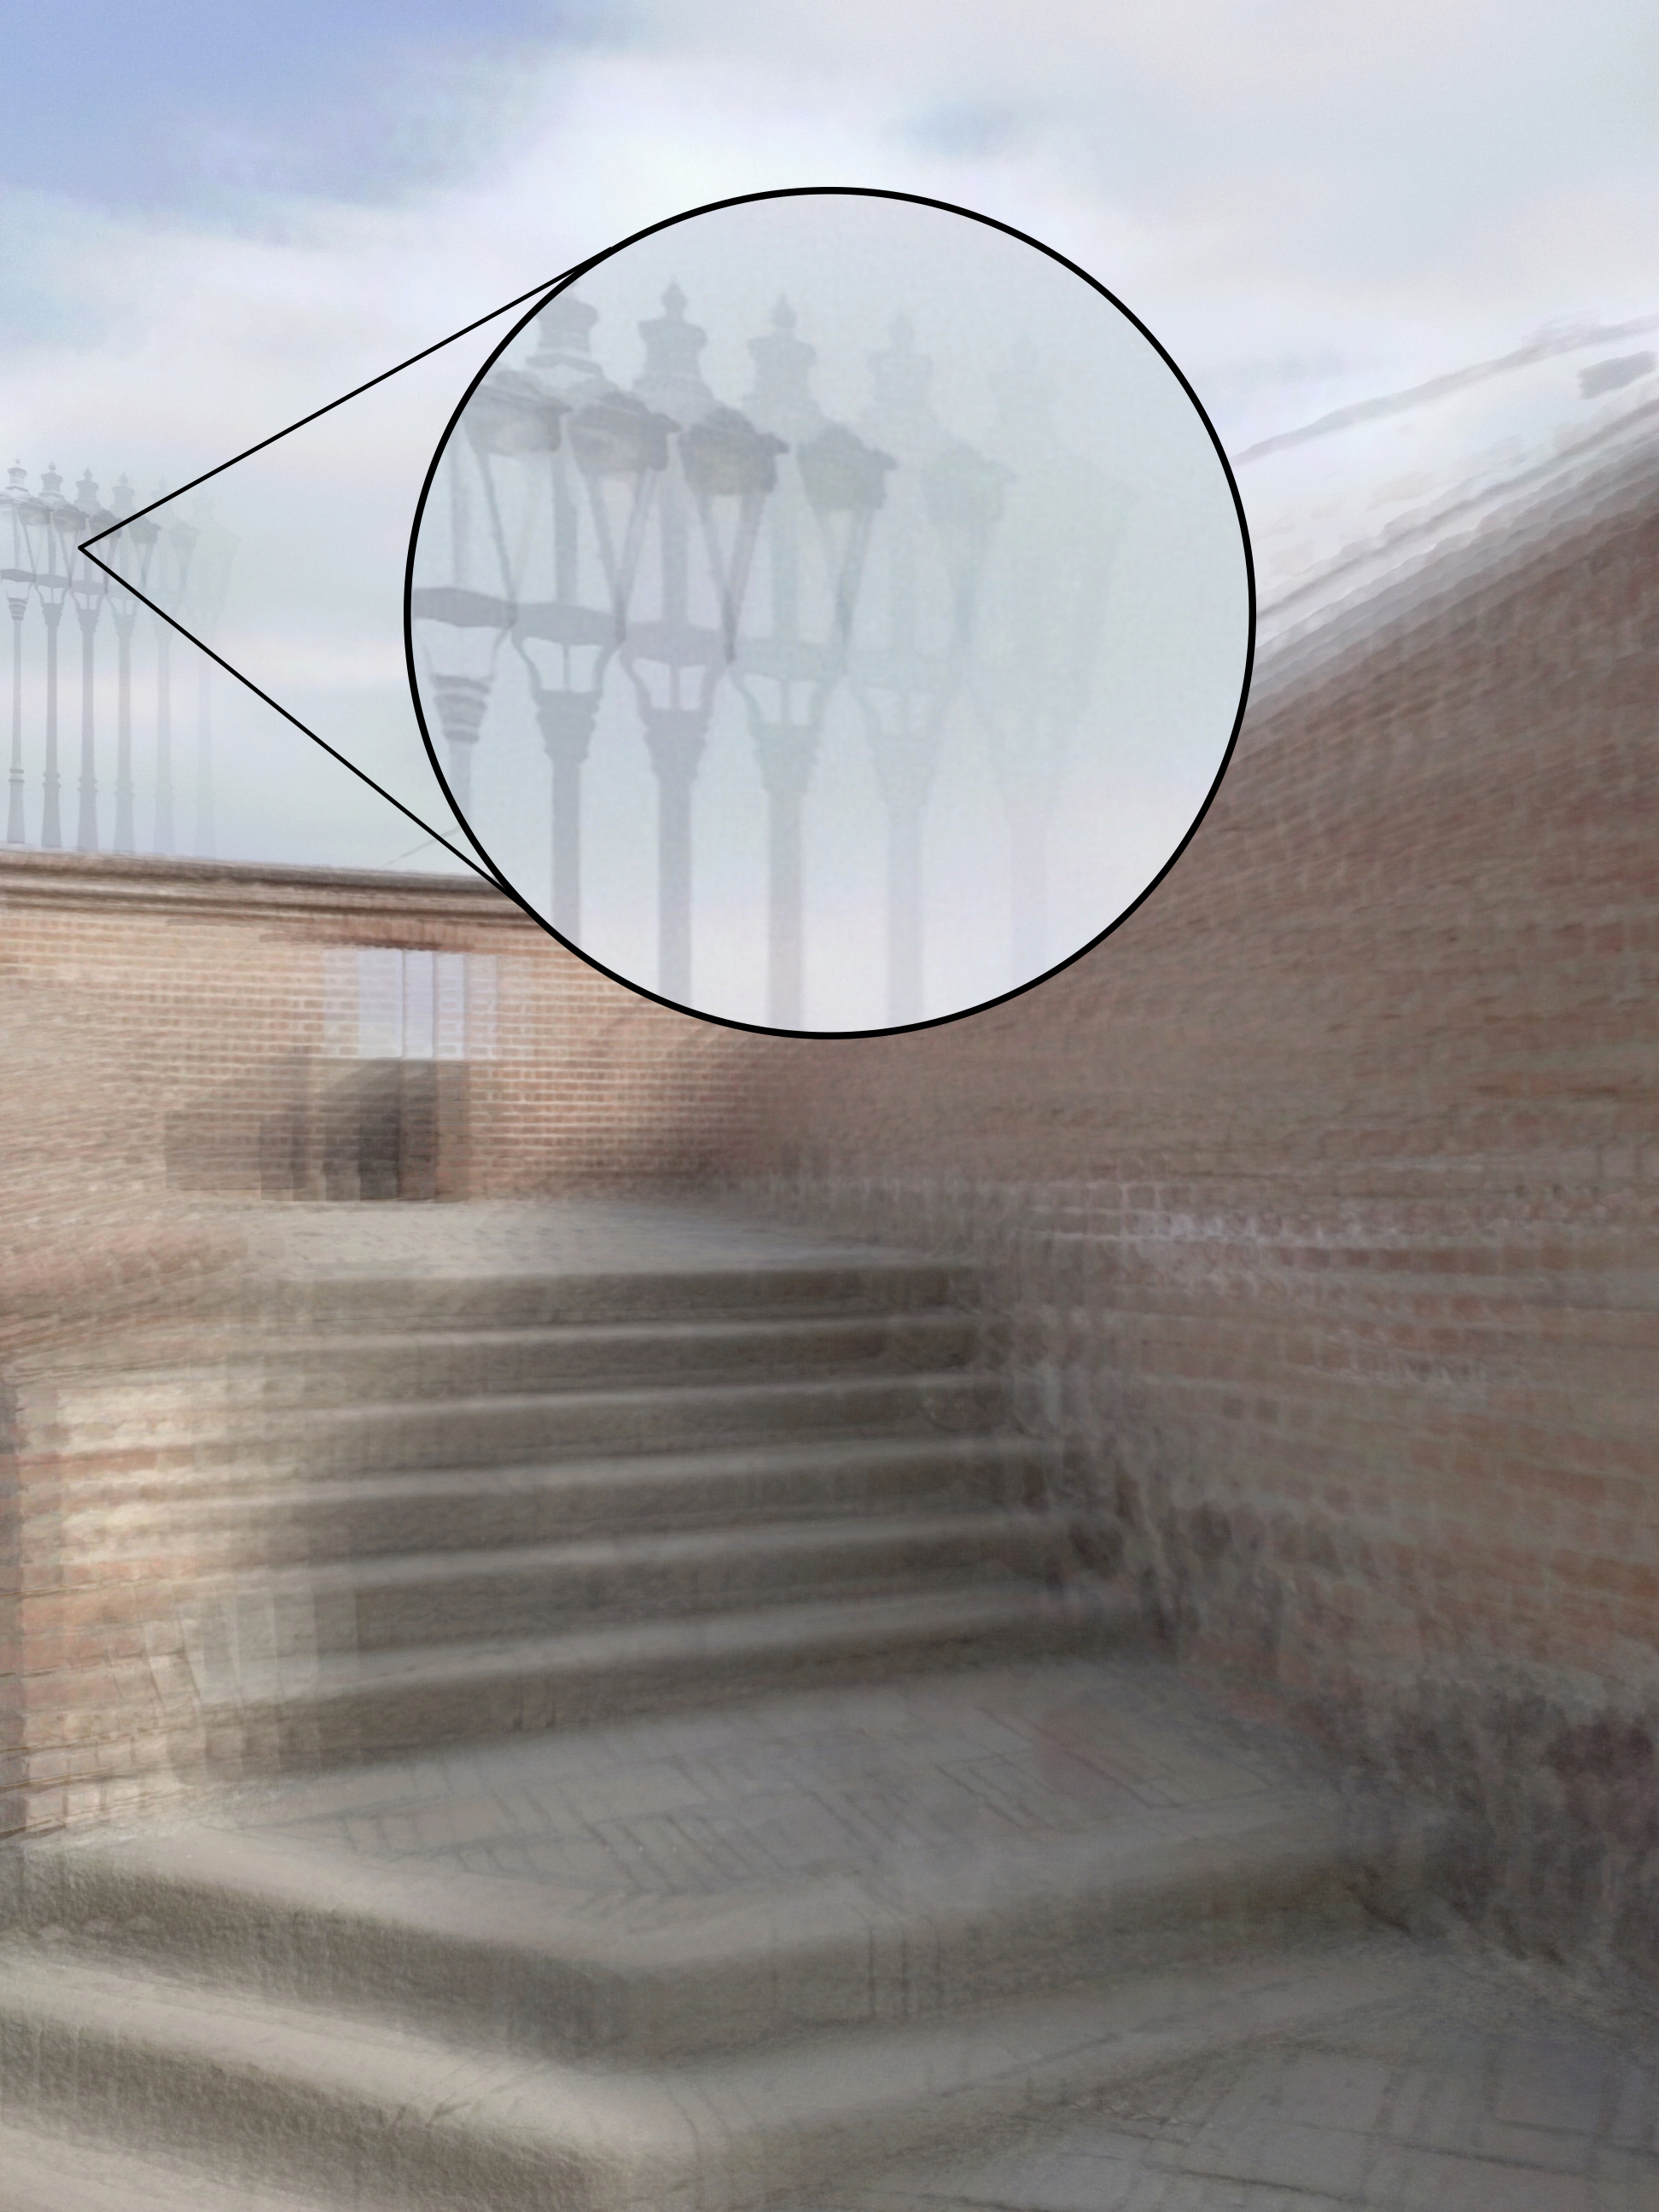
\includegraphics[width=0.3\textwidth]{figures/capturing/align/unaligned}
    \caption{Problémy vznikajúce pri nezarovnaní snímok}
    \label{fig:unaligned}
\end{figure}

\subsection*{Median threshold bitmap}

Pre zarovnanie vytvorených snímok je použitá metóda Grega Warda (2003), implementovaná v triede
\texttt{AlignMTB} knižnice OpenCV.

Vstupom metódy je zoznam vytvorených snímok, ktoré sú váženým priemerom prevedené na obrázky v stupňoch šedej.
Podľa histogramu jasu obrázkov sa určí 8-bitová hodnota mediánu a vytvoria sa MTB obrazy, kde každý pixel, ktorý 
je jasnejší než medián, má hodnotu 1 a v opačnom prípade hodnotu 0 \cite{Align}.

Metóda nepracuje s expozíciou snímok. Na obrázku \ref{fig:mtb} môžeme vidieť, že MTB obrazy sú pre rôzne expozície
skoro identické. Obrázky naľavo predstavujú vybrané snímky zo série expozicií scény a napravo sú ich príslušné
MTB obrazy.

\begin{figure}[t]
    \centering
    \begin{subfigure}{0.3\textwidth}
        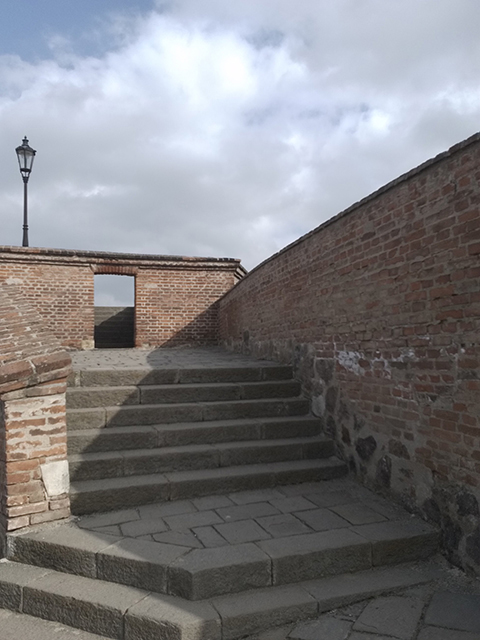
\includegraphics[width=\textwidth]{figures/capturing/align/image1}
    \end{subfigure}
    ~
    \begin{subfigure}{0.3\textwidth}
        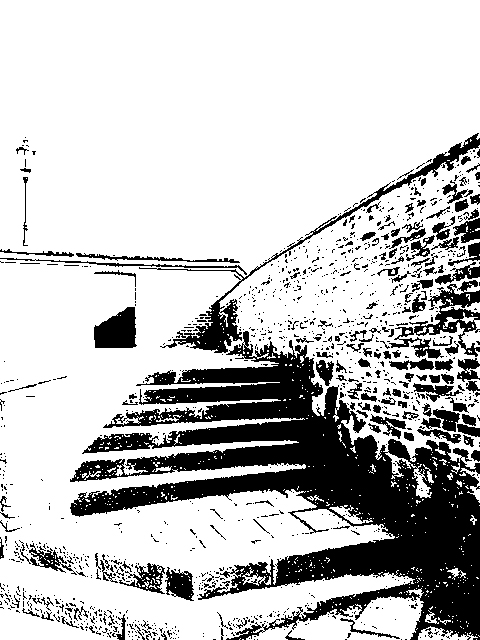
\includegraphics[width=\textwidth]{figures/capturing/align/image1tb}
    \end{subfigure}

    \begin{subfigure}{0.3\textwidth}
        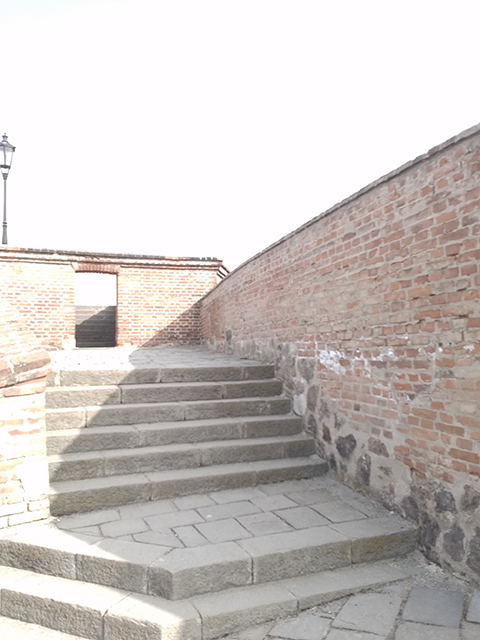
\includegraphics[width=\textwidth]{figures/capturing/align/image2}
    \end{subfigure}
    ~
    \begin{subfigure}{0.3\textwidth}
        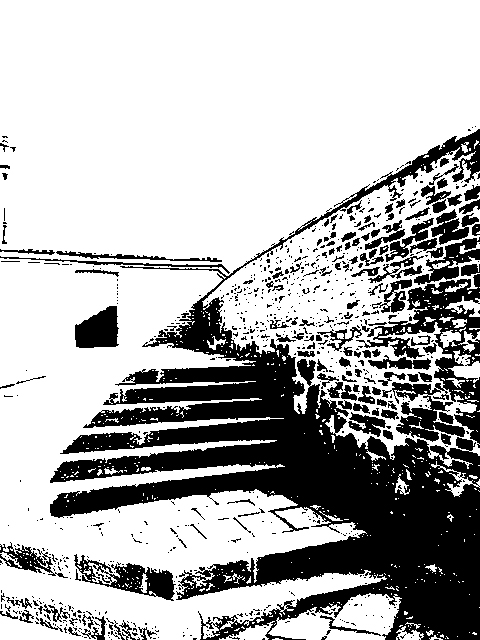
\includegraphics[width=\textwidth]{figures/capturing/align/image2tb}
    \end{subfigure}
    \caption{MTB obrazy vytvorené zo snímok z rozličným expozičným časom}
    \label{fig:mtb}
  \end{figure}

Jeden zo zoznamu obrázkov je zvolený za referenčný obrázok, podľa ktorého sa určujú číselné offsety zvyšných obrázkov.
Použitím XOR operátora môžeme na matici pixelov páru obrázkov jasne určiť offset nezarovnanosti na osiach $x$ a $y$.
Rýchlosť tejto metódy spočíva vo využívaní bitových operácií nad obrázkami, ktoré sú usporiadané v obrazovej pyramíde.
Offset sa začína určovať na páre obrázkov s najnižším rozlíšením. Postupne sa prechádza k~obrázkom s vyšším rozlíšením
a počíta sa odchýlka predchádzajúceho offsetu vynásobeného dvomi, čo zodpovedá zmene rozlíšenia.
Novovzniknuté oblasti obrazu sú vyplnené nulovými hodnotami.
